\documentclass[../differential_geometry.tex]{subfiles}
\begin{document}
\section{Aula 18 - 02 de Junho, 2026}
\subsection{Motivações}
\begin{itemize}
	\item Famílias de Curvas em Superfícies.
\end{itemize}
\subsection{Famílias de Curvas em Superfícies}
Continuemos de onde paramos.
\begin{example}[Superfícies de Revolução]
	Seja \(\underline{x}(u, v) = (f(v)\cos^{}{u}, f(v)\sin^{}{u}, g(v))\) uma parametrização local da superfície de revolução obtida girando a curva
	\[
		\alpha (v) = (f(v), 0, g(v))
	\]
	em torno do eixo z. Temos:
	\begin{align*}
		 & \underline{x}_{u} = (-f(v)\sin^{}{u}, f(v)\cos^{}{u}, 0),                                                                                                                                       \\
		 & \underline{x}_{v} = (f'(v)\sin^{}{u}, f'(v)\cos^{}{u}, g'(v)),                                                                                                                                  \\
		 & \underline{x}_{u} = (-f(v)\cos^{}{u}, -f(v)\sin^{}{u}, 0),                                                                                                                                      \\
		 & \underline{x}_{u} = (-f'(v)\sin^{}{u}, f'(v)\cos^{}{u}, 0),                                                                                                                                     \\
		 & \underline{x}_{vv} = (f''(v)\sin^{}{u}, f''(v)\cos^{}{u}, g''(v)),                                                                                                                              \\
		 & N = \frac{\underline{x}_{u}\times \underline{x}_{v}}{\Vert \underline{x}_u \times \underline{x}_v \Vert} = \frac{(g'(v)\cos^{}{u}, g'(v)\sin^{}{u}, -f'(v))}{\sqrt[]{(f')^{2}(v)+(g')^{2}(v)}}.
	\end{align*}
	Daí,
	\begin{align*}
		 & E = f^{2}(v), \quad \ell = - \frac{f(v)g'(v)}{\sqrt[]{(f')^{2}(v) + (g')^{2}(v)}}                                  \\
		 & F = 0, \quad m = 0                                                                                                 \\
		 & G = (f')^{2}(v) + (g')^{2}(v) \quad\&\quad n = \frac{f''(v)g'(v)-f'(v)g''(v)}{\sqrt[]{(f')^{2}(v) + (g')^{2}(v)}}.
	\end{align*}
	Uma direção \(a\underline{x}_u + b\underline{x}_v\) é principal se, e somente se,
	\[
		\det \begin{bmatrix}
			b^{2} & -ab & a^{2} \\
			E     & 0   & G     \\
			\ell  & 0   & n
		\end{bmatrix} = 0 \Longleftrightarrow (En - \ell G)ab = 0.
	\]
	Nos pontos onde \(En-\ell G \neq 0\), as soluções são \(a=0\) ou \(b=0\), ou seja, são \(\underline{x}_{u}\) e \(\underline{x}_v\). Portanto, as linhas de curvatura são as paralelas às meridianas.
\end{example}
\begin{def*}
	Uma curva \(\beta (t)\) em uma superfície \(S\subseteq \mathbb{R}^{3}\) é uma \textbf{curva assintótica} se \(\beta '(t)\) é uma direção assintótica em \(T_{\beta (t)}S\) para todo t. \(\square\)
\end{def*}
Em termos de uma parametrização local \(\underline{x}\) de S, tal que \(\beta (t) = \underline{x}(u(t), v(t))\), podemos caracterizar as curvas assintóticas como sendo aquelas com condição necessária e suficiente que
\[
	\mathbb{I}_{\beta (t)}(u'\underline{x}_u + v'\underline{x}_v) = 0 \Longleftrightarrow u^{2'}\ell +2u'v'm + v^{2'}n=0.
\]
\begin{example}
	Considere a superfície \(S: z = \frac{1}{2}(x^{2}-y^{2})\) parametrizada por
	\[
		\underline{x}(u, v) = (u+v, u-v, 2uv),
	\]
	com
	\[
		\ell =0,\; m=-\frac{2}{\sqrt[]{1+u^{2}+v^{2}}}, \;\&\; n =0.
	\]
	Então, \(\beta (t) = \underline{x}(u(t), v(t))\) é assintótica se, e somente se,
	\[
		u'v' = 0,
	\]
	que equivale a dizer que ou \(u\) é constante, ou \(v\) é constante.
	\begin{figure}[H]
		\begin{center}
			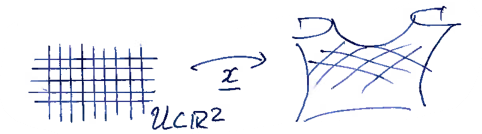
\includegraphics[height=\textheight, width=\textwidth, keepaspectratio]{./Images/curvature_to_saddle_18.png}
		\end{center}
	\end{figure}
\end{example}

Disto, surgem algumas perguntas:
\begin{itemize}
	\item[1)] Como as curvas assintóticas chegam à curva parabólica?
	\item[2)] Quais são as configurações da linha de curvatura ao redor dos pontos umbílicos?
\end{itemize}
Em geral, para superfícies parametrizadas num aberto denso, temos as seguintes configurações:

\begin{figure}[H]
	\begin{center}
		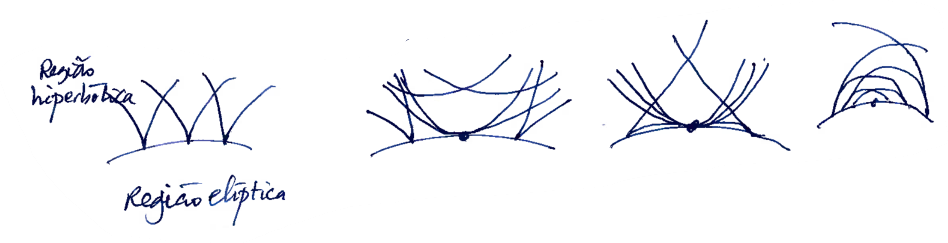
\includegraphics[height=\textheight, width=\textwidth, keepaspectratio]{./Images/stable_asymptotic_18.png}
		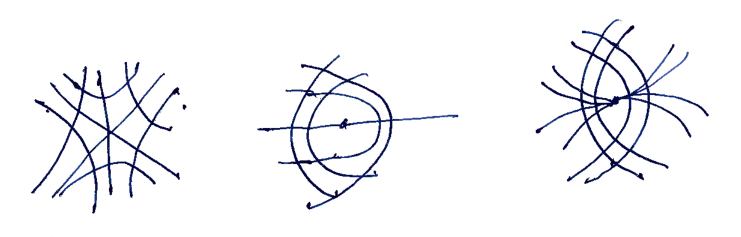
\includegraphics[height=\textheight, width=\textwidth, keepaspectratio]{./Images/stable_lines_18.png}
	\end{center}
	\caption{Na primeira linha da imagem, estão as configurações estáveis das curvas assintóticas; na segunda, as estáveis das linhas de curvatura!}
\end{figure}

\subsection{Alguns Resultados Globais}

\begin{def*}
	Diremos que uma superfície é \textbf{fechada} se ela for compacta e \textit{sem bordo}. \(\square\)
\end{def*}
\begin{theorem*}
	Toda superfície fechada em \(\mathbb{R}^{3}\) tem pelo menos um ponto elíptico.
	\begin{figure}[H]
		\begin{center}
			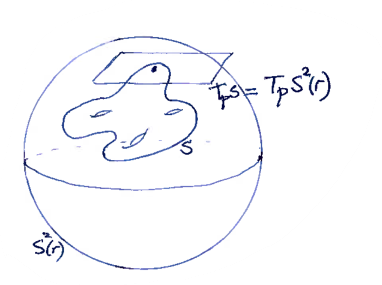
\includegraphics[height=\textheight, width=\textwidth, keepaspectratio]{./Images/closed_surfaces_18.png}
		\end{center}
	\end{figure}
\end{theorem*}
\begin{proof*}
	Seja \(f:\mathbb{R}^{3}\rightarrow \mathbb{R}\) dada pelo produto interno:
	\[
		f(x)\coloneqq \langle x, x \rangle,
	\]
	que sabemos ser diferenciável. Como S é compacta, existe um ponto \(p_{0}\) em S tal que seu máximo é atingido:
	\[
		f(p)\leq f(p_{0}), \quad \forall p\in S
	\]

	Agora, seja \(\alpha :(-\varepsilon , \varepsilon )\rightarrow S\) uma curva parametrizada por comprimento da arco, com \(\alpha (0) = p_{0}.\) A função \(f(\alpha (s))\) terá, então, um máximo local em \(S=0\), pois
	\[
		f(\alpha (s))\leq \varphi (\alpha (0))=f(p_{0}),
	\]
	e obtemos
	\[
		\frac{\mathrm{d}}{\mathrm{d}s}(f(\alpha (s))) = 2\langle \alpha '(s), \alpha (s) \rangle.
	\]
	Logo, em \(S=0,\) vale
	\[
		\langle \alpha '(0), \alpha (0) \rangle = \langle \alpha '(0), p_{0} \rangle = 0,
	\]
	para toda curva \(\alpha \) em S partindo de \(p_{0}\). Logo, o vetor normal a S em \(p_{0}\) é dado por
	\[
		N(p_{0}) = \frac{p_{0}}{\Vert p_{0} \Vert}.
	\]

	Como \(s=0\) é um máximo local de \(f(\alpha (s))\), temos
	\[
		\frac{\mathrm{d}^{2}}{\mathrm{d}s^{2}}(f\circ \alpha )(0)\leq 0,
	\]
	levando às relações
	\begin{align*}
		                    & \langle \alpha''(0), \alpha '(0) \rangle + \overbrace{\langle \alpha '(0), \alpha '(0) \rangle}^{=1}\leq 0 \\
		\Longleftrightarrow & \langle \alpha ''(0), p_{0} \rangle\leq -1                                                                 \\
		\Longleftrightarrow & \langle \alpha ''(0), \Vert p_{0} \Vert N(p_{0}) \rangle\leq -1                                            \\
		\Longleftrightarrow & \langle \alpha''(0), N(p_{0}) \rangle \leq -\frac{1}{\Vert p_{0} \Vert}<0.
	\end{align*}
	Daí, para todo \(\alpha '(0)\) em \(T_{p_{0}}S\), vale que
	\[
		\kappa_{n}(\alpha '(0)) < 0
	\]
	e, consequentemente,
	\[
		\kappa_1(p_{0}) < 0 \quad\&\quad \kappa_2 (p_{0}) < 0.
	\]
	Portanto, \(K(p_{0}) > 0\) e \(p_{0}\) é um ponto elíptico. \qedsymbol
\end{proof*}
\begin{crl*}
	Não existem superfícies fechadas em \(\mathbb{R}^{3}\) com \(K \leq 0\) em todos os seus pontos.
\end{crl*}
Outra ``consequência'', ainda não provada, é devido a Caratheodory em meados de 1924:
\begin{prop*}[Conjectura de Caratheodory]
	Toda superfície fechada e convexa tem pelo menos dois pontos umbílicos.
\end{prop*}

\subsection{Teorema Egreguim de Gauss: contexto e enunciado}
Seja S uma superfície em \(\mathbb{R}^{3}\) e \(\underline{x}:U\subseteq \mathbb{R}^{2}\rightarrow S\subseteq \mathbb{R}^{3}\) uma parametrização local de S. Conforme aprendemos, a curvatura Gaussiana de S é dada por
\[
	K = \frac{\ell n - m^{2}}{EG - F^{2}},
\]
onde os coeficientes E, F e G da primeira forma fundamental dependem da métrica \(\mathrm{d}s^{2}\) em S, que, neste caso, é dada pela restrição do produto escalar em \(\mathbb{R}^{3}\) a \(T_{p}S\) em cada ponto p de S.

\underline{\textit{No entanto}}, os coeficientes \(\ell ,\; n,\; m\) da segunda forma fundamental dependem do vetor normal N -- dependem do fato de que S mora em \(\mathbb{R}^{3}\); então, uma conclusão lógica é que a curvatura gaussiana depende do fato de que S mora em \(\mathbb{R}^{3}\), certo?

Na verdade, não! Gauss provou que, na verdade, depende apenas da primeira forma fundamental e de suas derivadas, ou seja, que \textbf{a curvatura gaussiana é intrínseca à curva}.

\hypertarget{egreguim_theorem}{
	\begin{theorem*}[Teorema Egreguim de Gauss]
		A curvatura gaussiana de uma superfície em \(\mathbb{R}^{3}\) depende somente dos coeficientes E, F, G e das suas derivadas.
	\end{theorem*}
}
Uma consequência deste teorema é que, como uma isometria local preserva a primeira forma fundamental, as isometrias locais preservam também a curvatura gaussiana! Esse resultado é muito poderoso; por exemplo, sabemos que existe uma isometria local entre o plano e o cilindo. Logo, a curvatura local do cilindro é nula, para qualquer ponto p
\begin{figure}[H]
	\begin{center}
		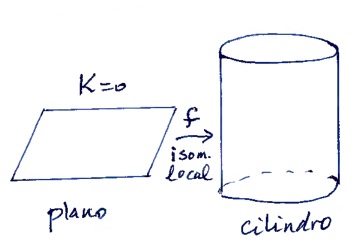
\includegraphics[height=0.7\textheight, width=0.7\textwidth, keepaspectratio]{./Images/plane_to_cylinder_19.png}
	\end{center}
\end{figure}
Outro exemplo é que sabemos que o plano tem curvatura Gaussiana \(K(p)\equiv0\) e que a esfera de raio r tem curvatura Gaussiana \(K(p) = \frac{1}{r^{2}}\), que é sempre não nula e positiva. Portanto, não existe isometria local entre o plano e a esfera!

\begin{tcolorbox}[
		skin=enhanced,
		title=Observação,
		fonttitle=\bfseries,
		colframe=black,
		colbacktitle=cyan!75!white,
		colback=cyan!15,
		colbacklower=black,
		coltitle=black,
		drop fuzzy shadow,
		%drop large lifted shadow
	]
	O \hyperlink{egreguim_theorem}{\textit{Teorema Egreguim}} não vale para a curvatura média
	\[
		H = \frac{1}{2}(\kappa_1 + \kappa_2);
	\]
	basta considerar caso do plano e do cilindro novamente: para o primeiro, \(H = 0\), mas, para o cilindro de base circular com raio r, \(H = \frac{1}{2r}\).
\end{tcolorbox}

\textbf{\underline{Curiosidade}:} a palavra Egreguim pode ser traduzida para ``egrégio'', ou ``importante'', e faz sentido, afinal a definição inicial da curvatura gaussiana faz uso da posição que a superfície ocupa no espaço, então realmente seria bem esperado que ela dependeria do espaço, mas acaba não dependendo!

Este resultado traz consequências bastante fundamentais; por exemplo, a falta de isometria entre uma esfera e uma reta pode parecer um resultado meio inocente, mas ele é traduzido no mundo real como ``não é possível fazer um mapa da Terra (aproximadamente esférica) sobre um mapa (plano), preservando todas as propriedades métricas dela.'' Toda projeção cartográfica terá alguma distorção!

\begin{def*}
	Os \textbf{símbolos de Christoffel} \(\Gamma_{ij}^{k}\) definem a ordem das derivadas em relação a u e a v (i e j), para cada derivada parcial de \(\underline{x}\), e qual coeficiente irá acompanhar (k)
\end{def*}
Por exemplo, se derivamos duas vezes em relação a u, então
\[
	\underline{x}_{{\color{DodgerBlue2}uu}} = \Gamma_{{\color{DodgerBlue2}11}}^{{\color{DarkGoldenrod1}1}}\underline{x}_{{\color{DarkGoldenrod1}u}} + \Gamma_{{\color{DodgerBlue2}11}}^{{\color{DarkOrchid4}2}}\underline{x}_{{\color{DarkOrchid4}v}} + \ell N
\]
e se derivarmos uma vez em v e outra em u, então
\[
	\underline{x}_{{\color{Chartreuse2}v}{\color{DodgerBlue2}u}} = \Gamma_{{\color{Chartreuse2}2}{\color{DodgerBlue2}1}}^{{\color{DarkGoldenrod1}1}}\underline{x}_{{\color{DarkGoldenrod1}u}} + \Gamma_{{\color{Chartreuse2}2}{\color{DodgerBlue2}1}}^{{\color{DarkOrchid4}2}}\underline{x}_{{\color{DarkOrchid4}v}}+mN
\]
\begin{proof*}[Prova do Teorema Egrégio]
	Precisamos provar que \(\ell n - m^{2}\) depende somente de \(E,\; F,\; G\) e de suas derivadas parciais em relação a u e v. Em cada ponto p de S, \(\underline{x}_u,\; \underline{x}_v, \; N\) formam uma base de \(\mathbb{R}^{3}\), fornecendo
	\[
		\underline{x}_{uu} = \alpha \underline{x}_u + \beta \underline{x}_v + \gamma N.
	\]
	Temos
	\[
		\langle \underline{x}_{uu}, N \rangle = \gamma = \ell .
	\]
	Usando a notação de Christoffel para escrever as derivadas duplas, temos:
	\begin{align*}
		 & \underline{x}_{{\color{DodgerBlue2}uu}} = \Gamma_{{\color{DodgerBlue2}11}}^{{\color{DarkGoldenrod1}1}}\underline{x}_{{\color{DarkGoldenrod1}u}} + \Gamma_{{\color{DodgerBlue2}11}}^{{\color{DarkOrchid4}2}}\underline{x}_{{\color{DarkOrchid4}v}} + \ell N                                                          \\
		 & \underline{x}_{{\color{Chartreuse2}v}{\color{DodgerBlue2}u}} = \Gamma_{{\color{Chartreuse2}2}{\color{DodgerBlue2}1}}^{{\color{DarkGoldenrod1}1}}\underline{x}_{{\color{DarkGoldenrod1}u}} + \Gamma_{{\color{Chartreuse2}2}{\color{DodgerBlue2}1}}^{{\color{DarkOrchid4}2}}\underline{x}_{{\color{DarkOrchid4}v}}+mN \\
		 & \underline{x}_{{\color{Chartreuse2}vv}} = \Gamma_{{\color{Chartreuse2} 22}}^{{\color{DarkGoldenrod1}1}}\underline{x}_{{\color{DarkGoldenrod1}u}} + \Gamma_{{\color{Chartreuse2} 22}}^{{\color{DarkOrchid4}2}}\underline{x}_{{\color{DarkOrchid4}v}}+mN                                                              \\
	\end{align*}
	Note que
	\[
		\Gamma_{12}^{1} = \Gamma_{21}^{1} \quad\&\quad \Gamma_{12}^{2}=\Gamma_{21}^{2}.
	\]

	Vamos calcular os símbolos de Christoffel: fazendo o produto escalar de \(\underline{x}_{uu}\) com \(\underline{x}_u\) e \(\underline{x}_v\), obtemos:
	\[
		\left\{\begin{array}{ll}
			\langle \underline{x}_u, \underline{x}_{uu} \rangle = \Gamma_{11}^{1}E + \Gamma_{11}^{2}F \\
			\langle \underline{x}_{v}, \underline{x}_{uu} \rangle = \Gamma_{11}^{1}F + \Gamma_{11}^{2}G
		\end{array}\right..
	\]
	Temos
	\[
		E = \langle \underline{x}_u, \underline{x}_u \rangle \Rightarrow \langle \underline{x}_u, \underline{x}_{uu} \rangle = \frac{1}{2}E_{u} \quad\&\quad \langle \underline{x}_u, \underline{x}_{uv} \rangle = \frac{1}{2}E_{v}
	\]
	e
	\[
		\langle \underline{x}_u, \underline{x}_v \rangle = F \Rightarrow \langle \underline{x}_{uu}, \underline{x}_v \rangle + \langle \underline{x}_u, \underline{x}_{uv} \rangle = F_{u}\\  \quad\&\quad \langle \underline{x}_v, \underline{x}_{uu} \rangle = F_{v}-\frac{1}{2}E_{v}.
	\]
	Logo,
	\[
		\left\{\begin{array}{ll}
			\Gamma_{11}^{1}E + \Gamma_{11}^{2}F = \frac{1}{2}E_{u} \\
			\Gamma_{11}^{1} F + \Gamma_{11}^{2}G = F_{v} - \frac{1}{2}E_{u}
		\end{array}\right.,
	\]
	e como \(EG-F^{2}> 0\), o sistema acima pode ser resolvida para \(\Gamma_{11}^{1}\) e \(\Gamma_{11}^{2}\), e as soluções dependem somente de E, F, G e das suas derivadas.

	Da mesma maneira, obtemos
	\[
		\left\{\begin{array}{ll}
			\Gamma_{12}^{1}E + \Gamma_{12}^{2}F = \frac{1}{2}E_{u} \\
			\Gamma_{12}^{1} F + \Gamma_{12}^{2}G = \frac{1}{2}G_{u}
		\end{array}\right., \quad\&\quad
		\left\{\begin{array}{ll}
			\Gamma_{22}^{1}E + \Gamma_{22}^{2}F = F_{v}-\frac{1}{2}G_{u} \\
			\Gamma_{22}^{1} F + \Gamma_{22}^{2}G = \frac{1}{2}G_{v}
		\end{array}\right.,
	\]

	Agora,
	\begin{align*}
		\ell n - m^{2} & =\langle \ell N, nN \rangle - \langle mN, mN \rangle                                                                                                                                            \\
		               & = \langle \underline{x}_{uu}-\Gamma_{11}^{1}\underline{x}_u - \Gamma_{11}^{2}\underline{x}_v, \underline{x}_{vv}-\Gamma_{22}^{1}\underline{x}_u - \Gamma_{22}^{2}\underline{x}_v \rangle        \\
		               & \quad\;- \langle \underline{x}_{uv}-\Gamma_{12}^1\underline{x}_{u} - \Gamma_{12}^{2}\underline{x}_v, \underline{x}_{uv}-\Gamma_{12}^{1}\underline{x}_u - \Gamma_{12}^{2}\underline{x}_v \rangle \\
		               & = \langle \underline{x}_{uu}, \underline{x}_{vv} \rangle - \langle \underline{x}_{uv}, \underline{x}_{uv} \rangle + \text{ termos de E, F, G e derivadas.}
	\end{align*}
	Porém,
	\begin{align*}
		\langle \underline{x}_{uu}, \underline{x}_{vv} \rangle - \langle \underline{x}_{uv}, \underline{x}_{uv} \rangle & = (\langle \underline{x}_{uu}, \underline{x}_{vv} \rangle + \langle \underline{x}_{u}, \underline{x}_{uvv} \rangle)-(\langle \underline{x}_{uv}, \underline{x}_{uv} \rangle + \langle \underline{x}_{u}, \underline{x}_{uvv} \rangle) \\
		                                                                                                                & =\frac{\partial^{}}{\partial u^{}}\langle \underline{x}_{u}, \underline{x}_{vv} \rangle - \frac{\partial^{}}{\partial v^{}}\langle \underline{x}_{u}, \underline{x}_{uv} \rangle                                                      \\
		                                                                                                                & =\frac{\partial^{}}{\partial u^{}}\biggl(F_{v}-\frac{1}{2}G_{u}\biggr)-\frac{\partial^{}}{\partial v^{}}\biggl(\frac{1}{2}E_{v}\biggr)                                                                                                \\
		                                                                                                                & = -\frac{1}{2}\biggl(E_{vv} - 2F_{uv} + G_{uu}\biggr).
	\end{align*}
	Portanto, os a curvatura gaussiana pode ser completamente descrita em termos de E, F, G e de suas derivadas. \qedsymbol
\end{proof*}
\end{document}

